\documentclass{sig-alternate}
%
%\usepackage{makeidx}  % allows for indexgeneration
%\usepackage[pdftex]{graphicx}\usepackage{graphicx}
\usepackage{float}
\usepackage{subfig}
\usepackage{caption}
\DeclareCaptionType{copyrightbox}
\usepackage{graphicx}
\usepackage{amsmath}
\usepackage{algorithm,algorithmicx}
\usepackage{algpseudocode}

\begin{document}
%\normalem


\title{Why so aggressive? Low Extra Delay Background Traffic (LEDBAT) in WebRTC}

\numberofauthors{3}

\author{
\alignauthor
Riccardo Reale\\
      \affaddr{Peerialism AB, Stockholm, Sweden}\\
      \email{riccardo@peerialism.com}
\alignauthor
Anton Blomberg\\
      \affaddr{Stockholm University, Stockholm, Sweden}\\
      \email{anton@naetet.se}
\alignauthor
Roberto Roverso\\
      \affaddr{Peerialism AB, Stockholm, Sweden}\\
      \email{roberto@peerialism.com}
}

\newcommand{\mysec}[1]{\vspace*{-0.0cm}\section{#1}}
\newcommand{\mysubsec}[1]{\vspace*{-0.0cm}\subsection{#1}\vspace*{0cm}}
\newcommand{\mysubsubsec}[1]{\vspace*{-0.0cm}\subsubsection{#1}\vspace*{0cm}}
\newcommand{\mypar}[1]{\vspace*{-0cm}\paragraph{#1}\vspace*{0cm}}

\maketitle
%\vspace*{-1cm}

\begin{abstract}
  In this paper, we present what is, to the best of our knowledge, the first
  implementation of LEDBAT for the WebRTC framework. By providing support for LEDBAT, we
  enable the development of data-intensive P2P applications on top of WebRTC, such as
  file-sharing and video streaming. This effort is a first step in the process of studying
  the functionality and performance of WebRTC in order to address the shortcomings that
  prevent wide adoption of the technology.
\end{abstract}

\category{C.2.2}{Computer-Communication Networks}{Network Protocols}
\category{C.2.4}{Computer-Communication Networks}{Distributed Systems}
\terms{Experimentation, Performance, Measurement}
\keywords{LEDBAT, WebRTC, Peer-to-peer}

\mysec{Introduction}
% WebRTC general 
Recently, WebRTC has been steadily gaining popularity fueled by the inclusion in most of
the browsers on the market. The WebRTC standard mandates the multimedia and peer-to-peer
connectivity stacks for real-time services, once provided by external plugins, to be built
directly into the browser. That means that features of those stacks, such as video
acquisition/encoding, encryption and NAT traversal, are made available to developers
through HTML5 APIs. WebRTC was mainly designed as a framework to facilitate video and
audio conferencing but it does include support for building other types of peer-to-peer
applications, such as CDN accellerators~\cite{peerCDN} and video streaming
platforms~\cite{nurminen2013p2p}.

% Why LEDBAT is important
Although WebRTC currently provides many features, it lacks support for low priority
transfers. Low priority is an essential requirement for P2P data-intensive applications,
e.g. Bittorrent and streaming platforms ~\cite{smoothcache}, which utilize this feature to
avoid disrupting traffic generated by both web browsing and low delay VoIP applications.
Support for low priority is provided in P2P network stacks by a delay-based congestion
control protocol such as LEDBAT~\cite{ledbat}. LEDBAT achieves low priority behaviour by
completely yielding to other TCP traffic on the same network and by keeping the delay on a
link fixed to a low and constant target.

% What we did 
In this paper, we present what is, to the best of our knowledge, the first implementation
of LEDBAT for the WebRTC framework. By providing support for LEDBAT, we enable the
development of data-intensive P2P applications on top of WebRTC. In our specific case
however, the interest in LEDBAT is motivated by the the needs of a commercial
peer-assisted streaming application called Hive Streaming~\cite{hive}. Hive utilizes low
priority traffic to prefetch data from other peers ahead of the playback deadline without
disrupting other traffic in the network.

In general, our target is to study the functionality and performance of WebRTC in order to
address the shortcomings that prevent wide adoption of this technology in a commercial
context. For that, besides adding support for low priority, we intend to analyse the
behavior of WebRTC's transport protocols in a variety of real use-cases and suggest
improvements to the same. In order to encourage the adoption of our contributions into the
standard WebRTC suite, we make the implementation of those open-source and available
at~\cite{webrtc-utp}.

% Given these initial results, we intend to continue to validate the behavior of our
% implementation of LEDBAT in WebRTC. Most importantly however, we will be concentrating our
% efforts in studying the efficiency of both SCTP and LEDBAT in the context of P2P
% data-intensive browser applications, invrstigating potential bottlenecks and proposing
% solutions to the current WebRTC stack.


% Open source


\begin{figure}[t]
  \centering
    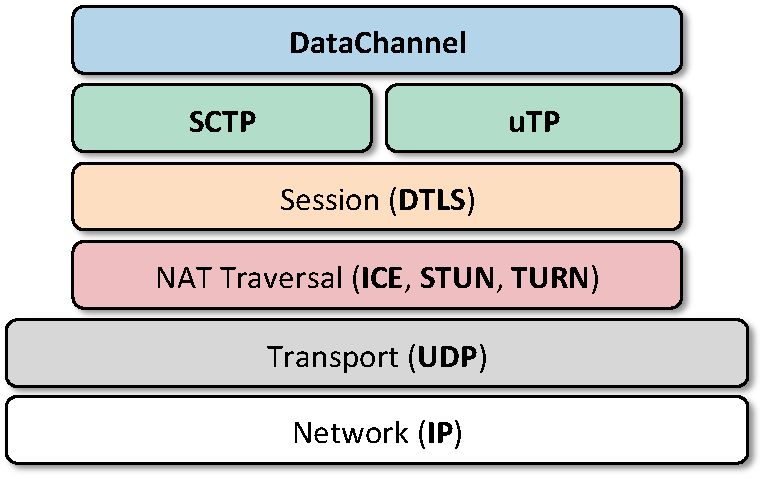
\includegraphics[width=0.30\textwidth]{figs/architecture3}
\vspace*{-0.38cm}
	\caption{WebRTC protocol stack} \label{fig:architecture}
\vspace*{-0.4cm}
\end{figure}

\mysec{LEDBAT in WebRTC}


In WebRTC, transfer of arbitrary data over encrypted P2P channels is a feature provided by
the DataChannel abstraction. 

% - how SCTP works
%The main reason why SCTP was chosen as application level transport protocol for the DataChannel is that it natively support some interesting features such as configurable in-order delivery, configurable reliability and a channel priority level defined by the application. Moreover it provides flow control and congestion control, while security is ensured by tunnelling all the traffic through a secure DTLS session, which itself run on top of UDP.


The DataChannel API make use of the Stream Control Transfer protocol (SCTP)~\cite{sctp}
protocol in order to manage data transfers. SCTP is message-oriented protocol that
provides a variety of options on data transfer to accomodate the needs of different types
of applications. When setting up a DataChannel, WebRTC applications may choose in- or
out-of-order delivery, reliable or unreliable delivery and have a specific priority level
on the channel. Regarding congestion control, the latest version of SCTP included in
WebRTC make use of the same algorithm found in H-TCP~\cite{htcp}. The main characteristic
of H-TCP is that it delivers the same priority as TCP in low bandwidth networks while
trying to better exploit high delay but large bandwidth links compared to TCP.

The current version of WebRTC's DataChannel incorporates a user-level SCTP
implementation~\footnote{http://sctp.fh-muenster.de/sctp-user-land-stack.html} written in \textit{C} and built
on top of UDP. SCTP interfaces with a security layer, DTLS, which adds security
and integrity to all traffic sent through a DataChannel session.  All data sent through
that session is carried over connections that have been established using the ICE NAT
Traversal protocol, last layer of the WebRTC protocol stack.


% - what we changed
In order to implement LEDBAT support in WebRTC, we opted to directly integrate the
\textit{uTP} library \cite{utp-repo} in the WebRTC protocol stack as an optional
alternative to SCTP. uTP is the reference open-source implementation of LEDBAT and is
provided by BitTorrent. Similarly to SCTP, uTP provides reliability, in-order delivery
and is layered over UDP. Given the similarities between the protocols, we were able to
easily integrate uTP with the existing WebRTC stack. That, by developing a translation
layer that interpret API requests from the DataChannel layer for the uTP layer. Besides
that, we modified the DataChannel API to be able to choose between SCTP and uTP as
transport protocol when setting up a data channel. The resulting structure of the WebRTC
stack is shown in Figure \ref{fig:architecture}. Finally, we were able to channel all data
processed by the uTP implementation into the DTLS processing.

\label{sec:architecture}

\mysec{Preliminary results}

% - setup
We conducted a preliminary evaluation of our solution in a controlled network environment
consisting of two host machines, a sender and a receiver, running Ubuntu Linux with kernel
3.11.0-12 connected by a 100 Mbps link. We used Dummynet on the sender host,
configured to cap the outgoing traffic to 1 Mbps, with 100 ms base delay and 60KB of queue
buffer to simulate a typical WAN gateway scenario. 

In order to test our implementation, we developed a test application in \textit{C} that
generates traffic using the WebRTC Native DataChannel API to emulate the traffic
of a data-intensive browser application. Our test application can be configured
to initialize either a STCP DataChannel, or a LEDBAT DataChannel.

Both hosts run our test application and a separate TCP traffic generator to obtain traffic
competing on the same network resources. TCP file transfer uses TCP Cubic, the default
Linux congestion control. Finally, a third host acts as a server to handle the WebRTC
session signalling between the sender and the receiver.

% - metrics
As metrics, we utilize the throughput of the DataChannel LEDBAT transfers, when competing
against TCP traffic, and the Round Trip Time (RTT) measured on the link. With these two
metrics, we verify that LEDBAT transfers indeed yield to TCP and, at the same time, we
evaluate the relative increase on the one-way delay, which directly affects latency and,
therefore, web browsing responsiveness.

% - evaluation
Figure \ref{fig:2ledbat_tcp} shows the throughput evolution of two DataChannel LEDBAT
streams and a single TCP stream, starting at 60 seconds from each other. The corresponding
Round Trip Time is also shown above. The two LEDBAT flows, as expected, utilize all
available bandwidth, until they quickly and completely release the bottleneck in favour of
the higher priority TCP flow. The increase in the RTT due to the presence of LEDBAT flows
is limited to 100 millisecond, which is the default target delay configuration in
uTP. Note that the number of LEDBAT streams doesn't affect the amount of extra delay
introduced.

%During the initial two minutes of the experiment, the LEDBAT streams correctly use all the available network resources while maintaining the introduced extra delay to a maximum of 100 millisecond, correspondent to the default target delay configured in uTP. At second 120 the two streams quickly release resources in favour of the higher priority TCP flow until it terminates. 

For direct comparison and validation that the normal behavior of SCTP was not affected,
Figure \ref{fig:2sctp_tcp} shows the same experiment performed configuring our test
application to use DataChannel SCTP streams. Besides fairly sharing the link with the TCP
transfer as expected, each of the SCTP streams introduce a large amount of extra-delay on
the link as TCP does.

\begin{figure}[t]
  \centering
    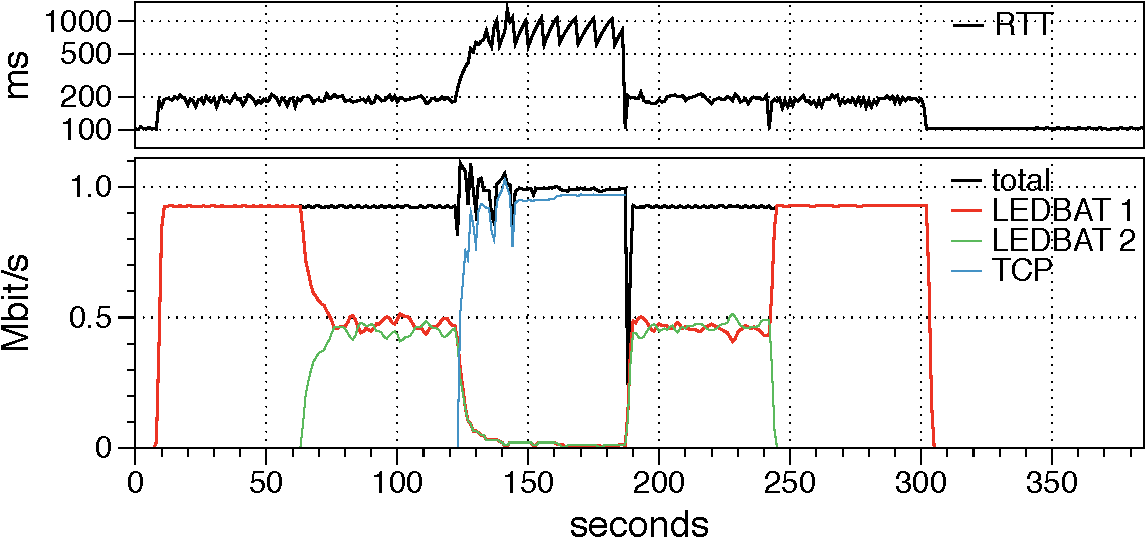
\includegraphics[width=0.47\textwidth]{figs/2ledbat_tcp}
\vspace*{-0.38cm}
	\caption{Two DataChannel LEDBAT streams sharing a 1Mbit/s bottleneck with a TCP stream} \label{fig:2ledbat_tcp}
%\vspace*{-0.4cm}
\end{figure}

\begin{figure}[t]
  \centering
    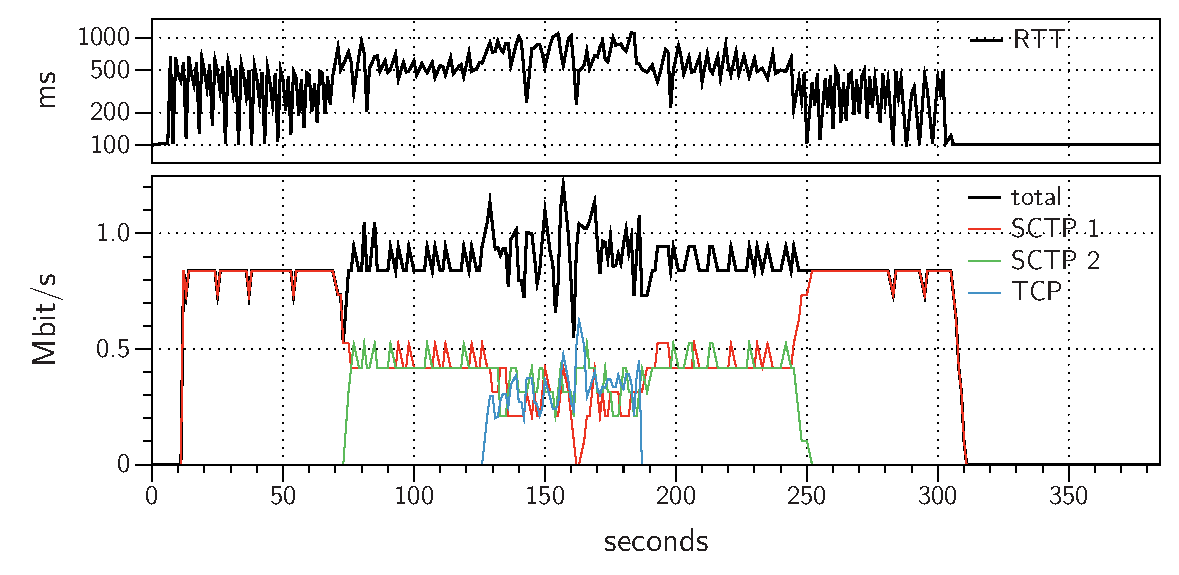
\includegraphics[width=0.47\textwidth]{figs/2sctp_tcp}
\vspace*{-0.38cm}
	\caption{Two DataChannel SCTP  streams sharing a 1Mbit/s bottleneck with a TCP stream} \label{fig:2sctp_tcp}
\vspace*{-0.4cm}
\end{figure}

\bibliographystyle{abbrv}
\bibliography{main}


\end{document}
